\documentclass[../main/main.tex]{subfiles}

\begin{document}

\section{Overview of exercises}

\begin{enumerate}
\item limb-darkening scattering exercise we did during the course. 
— You can look into your notes from that, and I attach here also a sample program which you can use a base. After you have familiarised yourself with this, you can start to think bout how you would go about to extend this to a 3D setting (assuming isotropic scattering). 

\item (As prep for Monte-Carlo school) here is a script computing a UV resonance P-Cygni line in spherically symmetric wind with v beta-law. At top of routine, a few exercises are given, where you can modify and play around with code. Monte-Carlo program which computes a UV resonance spectral line from a fast outflowing spherically symmetric stellar wind (if you were not cc’d on that email, let me know so that I can send you the files as well). At the top of that little script, there are a few suggestions for exercises (additions) you could do to that program, in order to learn a bit more about the general workings of Monte-Carlo radiative transfer in this context.  
— So that might be a good idea for you to do as well !   (And you can also ask the others in the group for some tips etc. then.) 

\item Some background reading: 
\begin{itemize}
\item Attached mc manual by Puls. 
\item Paper by Sundqvist+ 2010 (Appendix, I think). 
\end{itemize}

\end{enumerate}

\newpage
\section{Limb darkening}

\label{limb_darkening_discussion}

\subsubsection{2D Case}
We again have $\mu = \cos(\theta)$. The solution of the radiative transfer equation in \underline{plane-parallel syummetry} with frequency-independent absorption and emission, is 
\begin{equation}
I(\mu) = I_1 (0.4 + 0.6\mu)
\end{equation}
In the Monte Carlo code, the photons are sorted according to the direction that they leave the atmosphere.

\paragraph{Goal}
Calculates the angular dependence of photon's emitted from a plane-parallel, grey atmosphere of radial optical depth \texttt{taumax}. The value of \texttt{tau} determines the position of the photon

\paragraph{Variables and Algorithm}
\begin{itemize}
\item \texttt{muarray} contains emergent photons
\item \texttt{na} number of channels
\item \texttt{dmu} = 1/\texttt{na} width of channels
\item \texttt{nphot} number of photons
\item \texttt{taumax} maximum optical depth
\end{itemize}

\begin{algorithm}
\caption{Limb darkening: compute quantitiy of photons}\label{limb_darkening}
\begin{algorithmic}
\State initialization \\
\quad radial optical depth $\tau$ \\
\quad direction $\mu$

\For{all photons} 

\State $\boxed{\tau = \tau_{max}}$
	\While{\texttt{tau} $\geq 0$} 
	
	\State compute scattering angle \texttt{mu}
	\If{tau $\geq$ taumax} $\boxed{mu = sqrt(x)}$ (initial distribution)
	\Else{ $\boxed{mu = 2*x = 1}$} (isotropic scattering)
	\EndIf
	
	\State tau\_i = -log(x2) 
	\State tau = tau - tau\_i*mu	
		
	\EndWhile
	\State \textbf{end while}

	\State now we know that the photon has left the photosphere	
	\State compute the distribution of all angles \texttt{mu} at which the photon left the photosphere
	
\EndFor
\State \textbf{end for}

\State visualisation: 
	\begin{itemize}
	\item plot photon numbers from $\mu d\mu$ against \texttt{mu}
	\item plot specific intensity from $d\mu$ against \texttt{mu} against 
	\end{itemize}


\end{algorithmic}
\end{algorithm}


\begin{figure}[!htp]
\centering
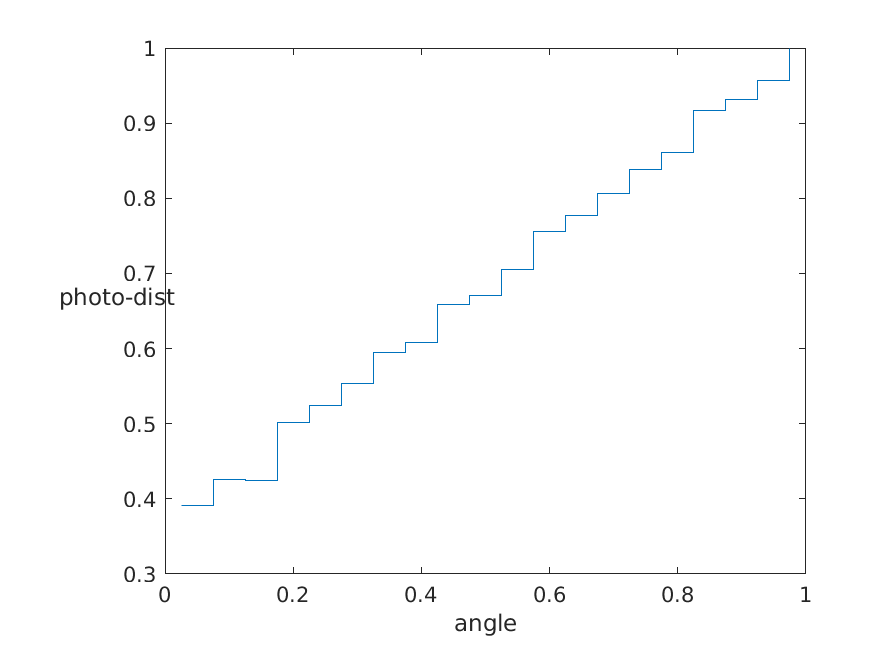
\includegraphics[width=0.7\textwidth]{../../introductory_exercises/limb_darkening/number_channels20number_photons100000max_opt_depth10.png}
\caption{histogram for \texttt{mu}}
\label{2D_mu}
\end{figure}
Figure \ref{2D_mu} is according to what is expected $I = I_0(0.4+0.6\mu)$

\newpage
\subsubsection{3D Code}
What changes is this: 
\begin{itemize}
\item introduction of a new angle $\phi$
\item the optical depth has to be updated according to $\phi$ also
\end{itemize}

\begin{figure}[!htp]
\centering
\begin{minipage}{.5\textwidth}
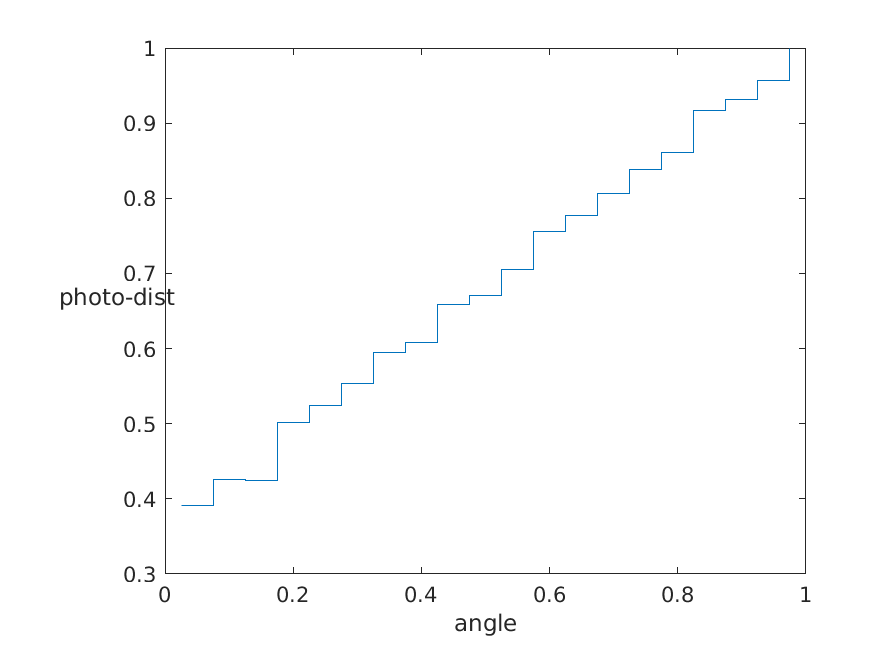
\includegraphics[width=\textwidth]{../../introductory_exercises/limb_darkening/number_channels20number_photons100000max_opt_depth10.png}
\caption{histogram for \texttt{mu}}
\label{3D_mu}
\end{minipage}%
\begin{minipage}{.5\textwidth}
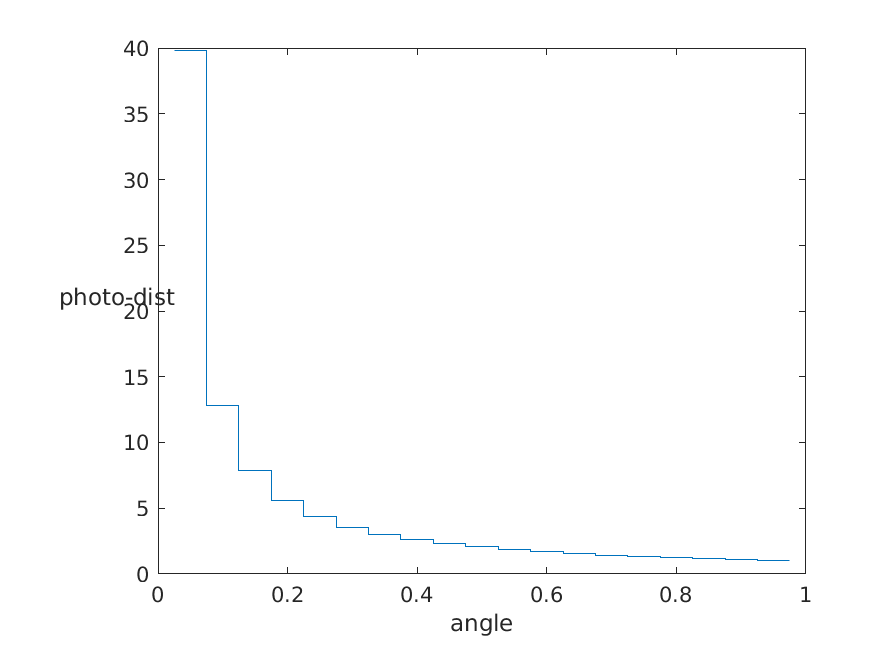
\includegraphics[width=\textwidth]{../../introductory_exercises/limb_darkening/PHI_number_channels20number_photons100000max_opt_depth10.png}
\caption{histogram for \texttt{phi}}
\label{3D_phi}
\end{minipage}
\end{figure}

Figure \ref{3D_mu} and Figure \ref{3D_phi} are according to what is expected, namely $I = I_0(0.4+0.6\mu)$ and a uniform distribution for $phi$, which corresponds to a $I \sim \frac{1}{\phi}$


\newpage
\section{Investigation of program: pcyg.f90}
\subsection{Overview of variables}
\begin{center}
\centering
{\tabulinesep=1.5mm
\begin{tabu}{|c|c|c|}
\hline 
name & explanation & scope \\ \hline \hline

\multicolumn{3}{|c|}{\cellcolor{orange} paramaters} \\ \hline
xk0 & \\ \hline
alpha & \\ \hline
beta & \\ \hline \hline

\multicolumn{3}{|c|}{\cellcolor{orange} start frequency of the photon} \\ \hline
xstart & start frequency & \\ \hline
vmin & & \\ \hline
vmax  & & \\ \hline

\multicolumn{3}{|c|}{\cellcolor{orange}angle of the photon} \\ \hline
xmuestart & start angle \\ \hline
xmuein & incident angle \\ \hline
xmueou & outward angle \\ \hline
\cellcolor{yellow} pstart & impact parameter \\ \hline
xnew & new photon frequency \\ \hline \hline

\multicolumn{3}{|c|}{\cellcolor{orange} optical depth} \\ \hline
tau & optical depth \\ \hline

\multicolumn{3}{|c|}{\cellcolor{orange} number of photons admin} \\ \hline
nphot & number of photons \\ \hline
nin & photons scattered back into core & \\ \hline
nout & photons escaped & \\ \hline \hline

\multicolumn{3}{|c|}{\cellcolor{orange} functions} \\ \hline
func & velocity profile \\ 
	& r & distance from center of star \\ \hline
	
xmueout & sign of outwards angle & \\ 
& xk0 & \\ 
& alpha & \\ 
& r & \\ 
& v & \\ 
& sigma & \\ \hline
\end{tabu}}
\end{center}

\newpage
\subsection{Exercises (at top of program)}
\subsubsection{Investigation of original code}
In original version of the code, all photons are released radially from photosphere, thus $\texttt{xmuestart} = 1$

\begin{figure}[!htp]
\centering
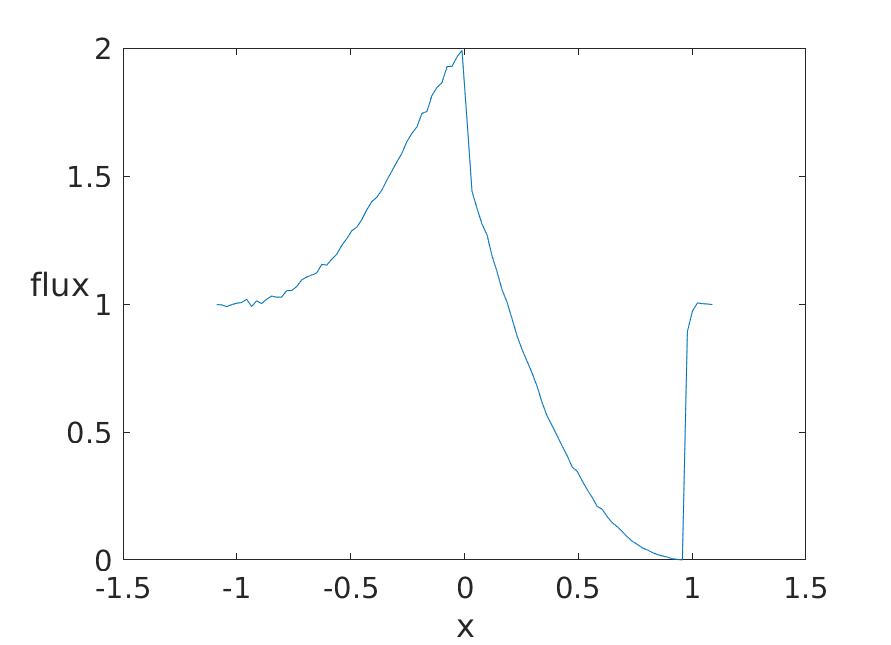
\includegraphics[width=0.5\textwidth]{../../introductory_exercises/P_Cygni_profile_UV_resonance/npot6xk0100alpha0beta1test0.png}
\caption{Original version of the code}
\end{figure}

\newpage
\subsubsection{First adaptation: what if all photons are released radially from photosphere?}
What would happen with line-profile, if you assumed all photons
!were released radially from photopshere?
\begin{itemize}
\item test case number 1
\item The code sets $mu = 1$. Results in Figure \ref{PCyg_mu=1}.
\end{itemize}


\begin{figure}[!htbp]
\centering
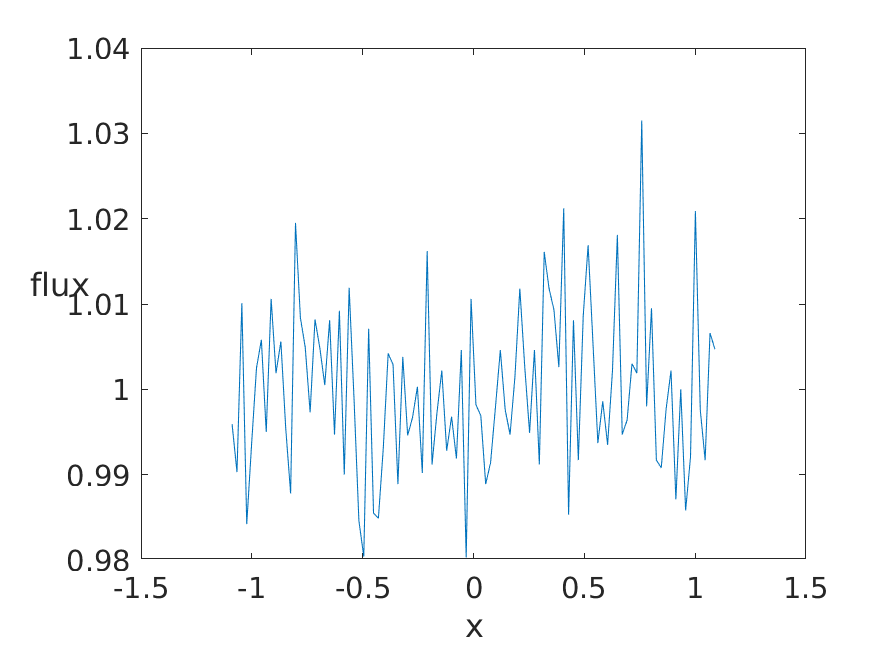
\includegraphics[width=0.5\textwidth]{../../introductory_exercises/P_Cygni_profile_UV_resonance/npot6xk0100alpha0beta1test1.png}
\caption{First adaptation}
\label{PCyg_mu=1}
\end{figure}

\newpage
\subsubsection{Second adaptation: isotropic scattering}
What would happen to line-profile, is you assumed scattering
!was isotropic (i.e., NOT following Sobo-distrobution)
\begin{itemize}
\item test case number 2
\end{itemize}

\begin{figure}[!htp]
\centering
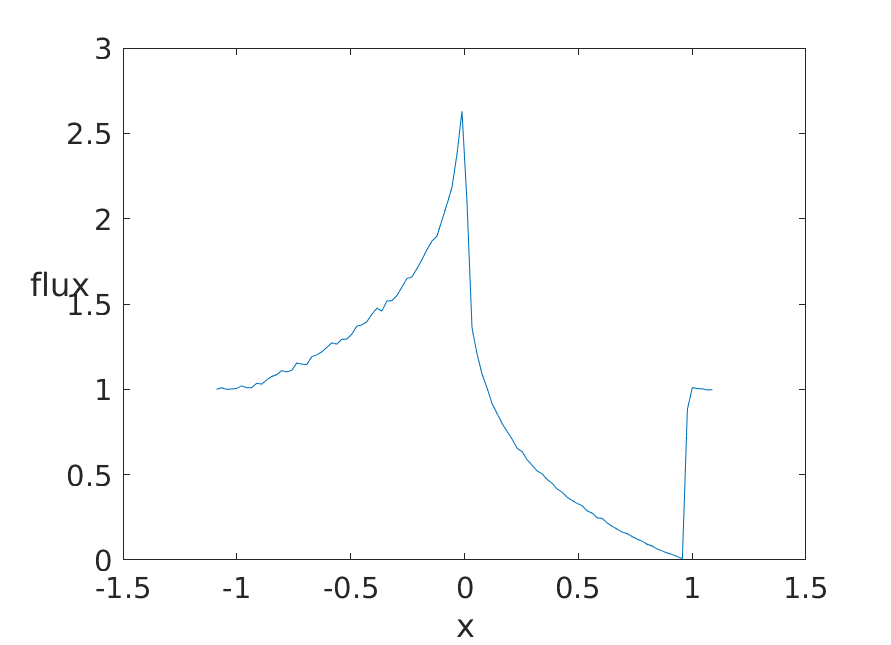
\includegraphics[width=0.5\textwidth]{../../introductory_exercises/P_Cygni_profile_UV_resonance/npot6xk0100alpha0beta1test2.png}
\caption{Second adaptation}
\end{figure}

The \textit{grosso modo} form has not changed, although the scaling has changed.

\newpage
\subsubsection{Third adaptation: introduction of Eddington limb-darkening}
Put Eddington limb-darkening in. What happens? 

\paragraph{General discussion: Eddington limb darkening}
The data are taken from Christensen, 2015.
\begin{itemize}
\item the source function $S= <I> = a + b\tau_{\nu}$ with $a= \frac{\sigma}{2 \pi}T_{eff}^4$ and $b = \frac{3 \sigma}{4 \pi}T_{eff}^4$
\item solve the equation
\item this yields $\frac{I(\theta)}{I(0)} = \frac{a+b\cos(\theta)}{a+b} = \frac{2}{5} + \frac{3}{5}\cos(\theta)$
\end{itemize}
\begin{figure}[!htp]
\centering
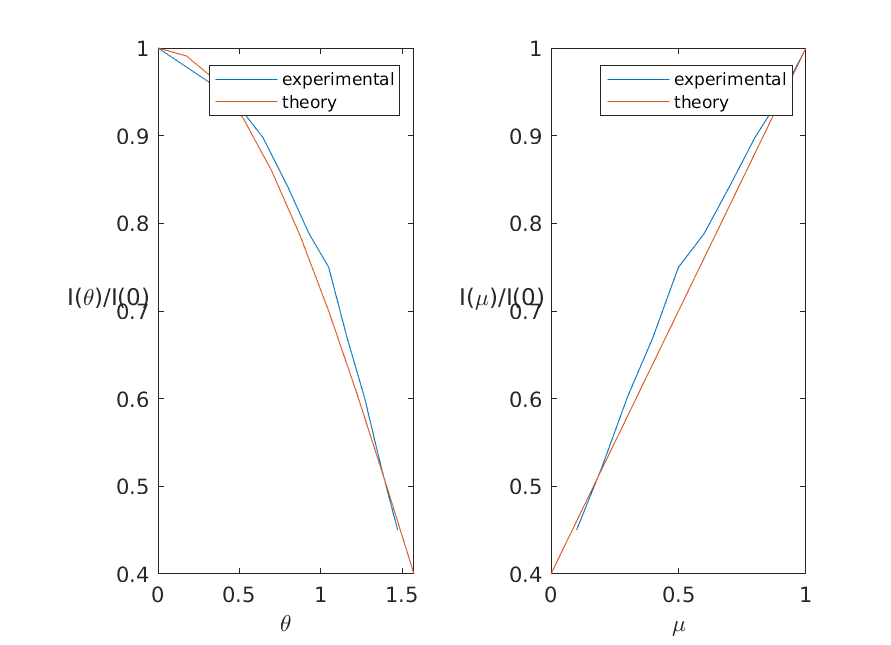
\includegraphics[width=0.7\textwidth]{../../introductory_exercises/P_Cygni_profile_UV_resonance/Eddington_limb_darkening.png}
\caption{Eddington limb darkening (two times the same plot with $\mu =  \cos(\theta)$ }
\end{figure}

\noindent\fbox{
  \parbox{\textwidth}{
for which star are the exerpimental data and what assumptions are used in the theory?
}}

\paragraph{Application to exercise}
\begin{itemize}
\item test case number 3 (not yet implemented)
\end{itemize}

\newpage
\subsubsection{Fourth adaptaion: photospheric line-profile}
Challening: Put photospheric line-profile (simple Gaussian) in
!What happens? Test on xk0=0 (opacity =0) case.

\begin{itemize}
\item test case number 4 (not yet implemented)
\end{itemize}


\newpage
\section{Mass loss from inhomogeneous hot star winds (Sundqvist)}
\begin{itemize}
\item GOAL: synthesis of UV resonance lines from inhomogeneous 2D winds
\begin{itemize}
\item clumped in density
\item clumped in velocity
\item effects of non-void inter-clump medium
\end{itemize}

\item WIND MODELS
\begin{itemize}
\item symmetry assumptions
\begin{itemize}
\item 1D: spherical symmetry
\item 2D: symmetry in $\Phi$
\end{itemize}

\item models
\begin{enumerate}

\item time-dependent radiation-hydrodynamic from Puls and Owocki (POF)
\begin{itemize}
\item 1D
\item isothermal flow
\item perturbations triggered by photospheric sound waves
\end{itemize}

\item time-dependent radiation-hydrodynamic from Feldmeier (FPP)
\begin{itemize}
\item 1D
\item treatment of energy equation
\item perturbations triggered by photospeheric sound waves or Langevin perturbagions (photospheric turbulence)
\end{itemize}

\item stochastic model, clumped in density
\begin{itemize}
\item smooth winds with $v_{\beta} = (1-b/r)^{\beta}$ with $\beta = 1$
\item clumping factor $f_{cl}$
\end{itemize}

\item stochastic model, clumped in density and in velocity (non-monotonic velocity field)
\begin{itemize}
\item smooth winds with $v_{\beta} = (1-b/r)^{\beta}$ with $\beta = 1$
\item clumping factor $f_{cl}$
\end{itemize}
\end{enumerate}

\end{itemize}

\item RADIATIVE TRANSFER (MC-2D)
\end{itemize}

\newpage
\section{Asymptotic preserving Monte Carlo methods for radiative transfer equation in diffusion limit (Dimarco+ 2018)}
\subsection{Goldstein-Taylor}
\subsection{Radiative transfer}

\end{document}